
% !TeX spellcheck = en_US

\chapter{Introduction to Flyway}

\section{Overview}
\marginpar{Information}%
Provide a detailed overview of the Flyway tool.\\


Flyway is a open source database migration tool. With flyway you can either write migration files with
SQL (database-specific syntax (such as PL/SQL, T-SQL, etc.) or Java (for advanced data transformations
or dealing with LOBs). It runs on all modern platforms such as Linux, Mac or Windows.
\cite{Dillon2022}, \cite{DBMSTools}



\marginpar{Features}%

\marginpar{Pro-Version}%

\marginpar{Advantages}%

\marginpar{Disadvantages}%
\begin{itemize}
	\item Important features like undo are only available in the paid Flyway Teams Edition.
\end{itemize}


\marginpar{Community}%
Stars on GitHub: 6'800 (31. October 2022)\\
Tags in StackOverflow: 2,088 (31. October 2022)\\

\newpage
\section{Functionality with Simplistic Example}
Explain how the Flyway tool works and provide a simplistic example to demonstrate.

\subsection{Installation and Setup}
Download the latest version of the \href{https://flywaydb.org/download/community}{Flyway Cummunity Edition} and extract the downloaded file. 
Once extracted, the file becomes a directory with the following structure:

\begin{figure}[H]
    \centering
    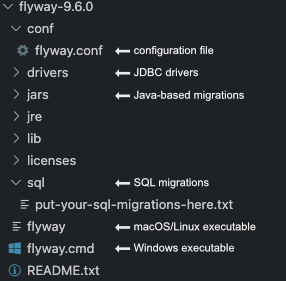
\includegraphics[width=0.4\textwidth]{./chapters/intro_flyway/images/flyway_folder_structure}
   \caption[Flyway folder structure - Source: Own illustration]{Flyway folder structure}
    % \label{fig:bsp_chapter:example_figure}
\end{figure}


\marginpar{Configuration}%
To connect to a running database, add the relevant information to \textit{conf/flyway.conf}.
In our minimal example this could be:

\begin{lstlisting}[caption=Minimal configuration]
flyway.url=jdbc:postgresql://localhost:5433/seminar
flyway.user=postgres
flyway.password=password
\end{lstlisting}

This is just a minimal configuration, but there are many more additional parameters that can be set \footnote{\url{https://flywaydb.org/documentation/configuration/parameters/}}.

\marginpar{SQL migrations}%
Flyway developers can migrate changes directly with SQL. Per default, flyway takes the database migrations from the directory \textit{sql}.
These SQL migration files have to follow the naming convention: \texttt{V<version number>\_\_<description>.sql}.

\begin{itemize}
    \item "V": This letter indicates it is a versioned migration. Flyway provides different types of migrations
    \item <version number>: Increasing version number of migrations
    \item \_\_: Then two underscores
    \item <description>: Short description of the migration
    \item Add a .sql extension
\end{itemize}

\marginpar{Workaround Mac OS}%


\subsection{Usage \& minimal Example}

\marginpar{CLI and commands}%
\textbf{Migrate}\\
To create a first migration, add a database change as sql file into the sql directory (see \autoref{fig:flyway_sql_scripts}).
In our minimal example, the file \texttt{V1\_\_create\_db.sql} looks like the following:

\begin{lstlisting}[language=SQL, caption=Create a database]
CREATE TABLE weather (
	city            varchar(80),
	temp_lo         int,           -- low temperature
	temp_hi         int,           -- high temperature
	prcp            real,          -- precipitation
	date            date
);
\end{lstlisting}

To apply the first migration, run: \texttt{flyway migrate}.
If the migration is successful, you will see the output below:
\begin{lstlisting}[caption=Flyway first migration success]
(base) marco@MacBook-Pro-von-Marco flyway-9.6.0 % flyway migrate
Flyway is up to date
Flyway Community Edition 9.6.0 by Redgate
See what's new here: https://flywaydb.org/documentation/learnmore/releaseNotes#9.6.0

Database: jdbc:postgresql://localhost:5433/seminar (PostgreSQL 14.5)
Successfully validated 1 migration (execution time 00:00.021s)
Creating Schema History table "public"."flyway_schema_history" ...
Current version of schema "public": << Empty Schema >>
Migrating schema "public" to version "1 - create db"
Successfully applied 1 migration to schema "public", now at version v1 (execution time 00:00.030s)
\end{lstlisting}

Now the table \textit{weather} has been created by flyway. There was also an additional metadata table (\textit{flyway\_schema\_history}) created with the first migration. This metadata table holds various information regarding the migration and their past.

If one want to update the database for example with data, just create a new script with the name e.g. \texttt{V2\_\_add\_data.sql} and run  \texttt{flyway migrate} again.

\begin{lstlisting}[language=SQL, caption=Create a database]
INSERT INTO weather VALUES ('Zurich', 10, 17, 0.25, '2022-10-30');
INSERT INTO weather VALUES ('Rapperswil', 8, 15, 0.25, '2022-10-30');
\end{lstlisting}

\begin{figure}[H]
	\centering
	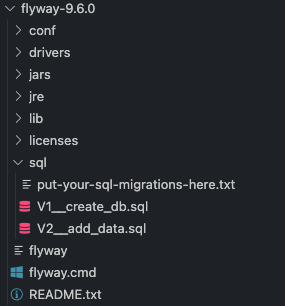
\includegraphics[width=0.4\textwidth]{./chapters/intro_flyway/images/flyway_v2_sql_migrations}
	\caption[Flyway SQL migrations - Source: Own illustration]{Flyway SQL migrations}
	 \label{fig:flyway_sql_scripts}
\end{figure}



In the following paragraph, a few very useful flyway commands are presented:\\
https://flywaydb.org/documentation/command/validate

\textbf{Info}\\
Get an overview of the applied migrations and their success status.\\

\textbf{Repair}\\
When a database migration fails, the migration is markes as failed in the schema history table (\textit{flyway\_schema\_history}). If a database supports DDL \footnote{Data Definition Language} transactions (like PostgreSQL), the failed migration is rolled back automatically and nothing is recorded in the schema history table.  But if the database does not support DDL transactions (e.g. Oracle Database, MySQL, MariaDB), you have two options to repair the database and remove the failed entries:

\begin{enumerate}
	\item Run \texttt{flyway repair}\\
	\item There are callbacks supported by flyway. One could use the \textit{afterMigrateError} and add a SQL-script to this callback, which deletes the failed migration entry in the \textit{flyway\_schema\_history} table.
	
	\begin{lstlisting}[language=SQL]
	DELETE IGNORE FROM flyway_schema_history WHERE success=0;
	\end{lstlisting}
\end{enumerate}

\textbf{clean}\\
With \texttt{flyway clean} one can drop all objects like tables, views, triggers, etc. in the configures schemas.It can easily give you a fresh start but is dangerous in a production environment.

\textbf{Validate}\\
If one want to be sure that all migrations are applied correctly,  \texttt{flyway validate} is the command of choice. The validation checks if the migration locally still has the same checksum as the migration executed in the database.
There is a possibility to apply custom validation rules. Because in a productive environment, there will be hotfixes, deleted migrations and other changes that break the default validation conventions (Flyway Teams Edition only).


\textbf{Undo}\\
To undo the most recent migration applied to the database, run \texttt{flyway undo}. The undo command can be repeated until the database is converted back to version 1.
Undo assumes that the previous applied migration succeeded and now should be undone. If the previsous applied migration failed, first repair the migrations before applying the undo-command. 
The undo-command is a Teams Edition feature only.

\textbf{Baseline}\\
This command makes the current database as the baseline for the future. This will cause Migrate to ignore all migration up to the actual version.
This can be useful to reduce the overhead, if you have many old migrations scripts that will not be used anymore.


\subsection{Usage with Java API, Maven or Gradle}
\marginpar{JavaAPI}%
LOBs,

\marginpar{Maven or Gradle}%
Integration with maven or gradle.
\newpage